%START TEXT INPUT
The Cracking Tool has to alter an application's behaviour by applying patches only to the \gls{apk} file, since it is the only source of code on the phone. This is the reason for the investigations to start with analysing the \gls{apk}. This is done using static analysis tools. The aim is to get an accurate overview of how the circumventing of the license verification mechanism is achieved. This knowledge is later used to find countermeasures to prevent the specific Cracking Tool from succeeding.\newline
The reengineering has to be done by using different layers of abstraction. The first reason is because it is very difficult to conclude from the altered bytecode, which is not human-readable, to the new behaviour of the application. The second reason is because the changes in the Java code are interpreted by the decompiler, which might not reflect the exact behaviour of the code or even worse, cannot be translated at all.\newline
These problems are encountered by analysing the different abstraction levels of code as well as different decompilers.
%START TEXT INPUT

%
recover the original code of an application bytecode analysis is most
often used. By applying both dynamic and static techniques to detect how behavior is altered\newline
dynamic analysis during runtime, static raw code, done by automatic tools using reverse engineering algorithms, best case whole code recovered, worst case none

When speaking of reverse engineering an Android application we mostly mean to reverse engineer the bytecode located in the dex file of this application.

The \textit{classes.dex} file is a crucial component regarding the application's code security because a reverse engineering attempt is considered successful when the targeted source code has been recovered from the bytecode analysis. Hence studying the DEX file format together with the Dalvik opcode structure is tightly related to both designing a powerful obfuscation technique or an efficient bytecode analysis tool.
\cite{kovachevaMaster}
%

%
dex to java
.dex and .class are isomorphic
dex debug items map dex offsets to java line numbers
tools like dex2jar can easily decomile from dex to a jar
extremly useful for reverse engineering, even more so useful for malice\newline
\begin{figure}[h]
    \centering
    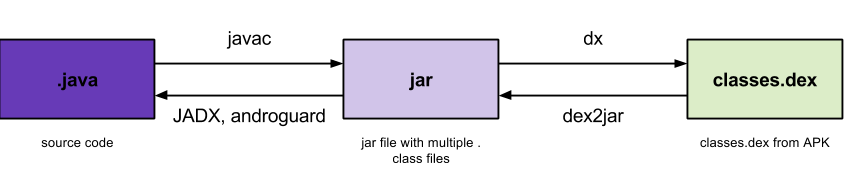
\includegraphics[width=0.8\textwidth]{data/re1.png}
    \caption{Java .class and .dex can be transformed bidirectional \cite{andevconDalvikART}}
    \label{fig:re1}
\end{figure}
flow from dex to java is bidirectional, decompile code back to java, remove annoyances like ads, registration, uncover sensitive data (app logic, secrets), replace certain classes with others (malicuous ones), recompile back to jar, then dex, put cloned/trojaned version of your app on play or other market\newline
\begin{figure}[h]
    \centering
    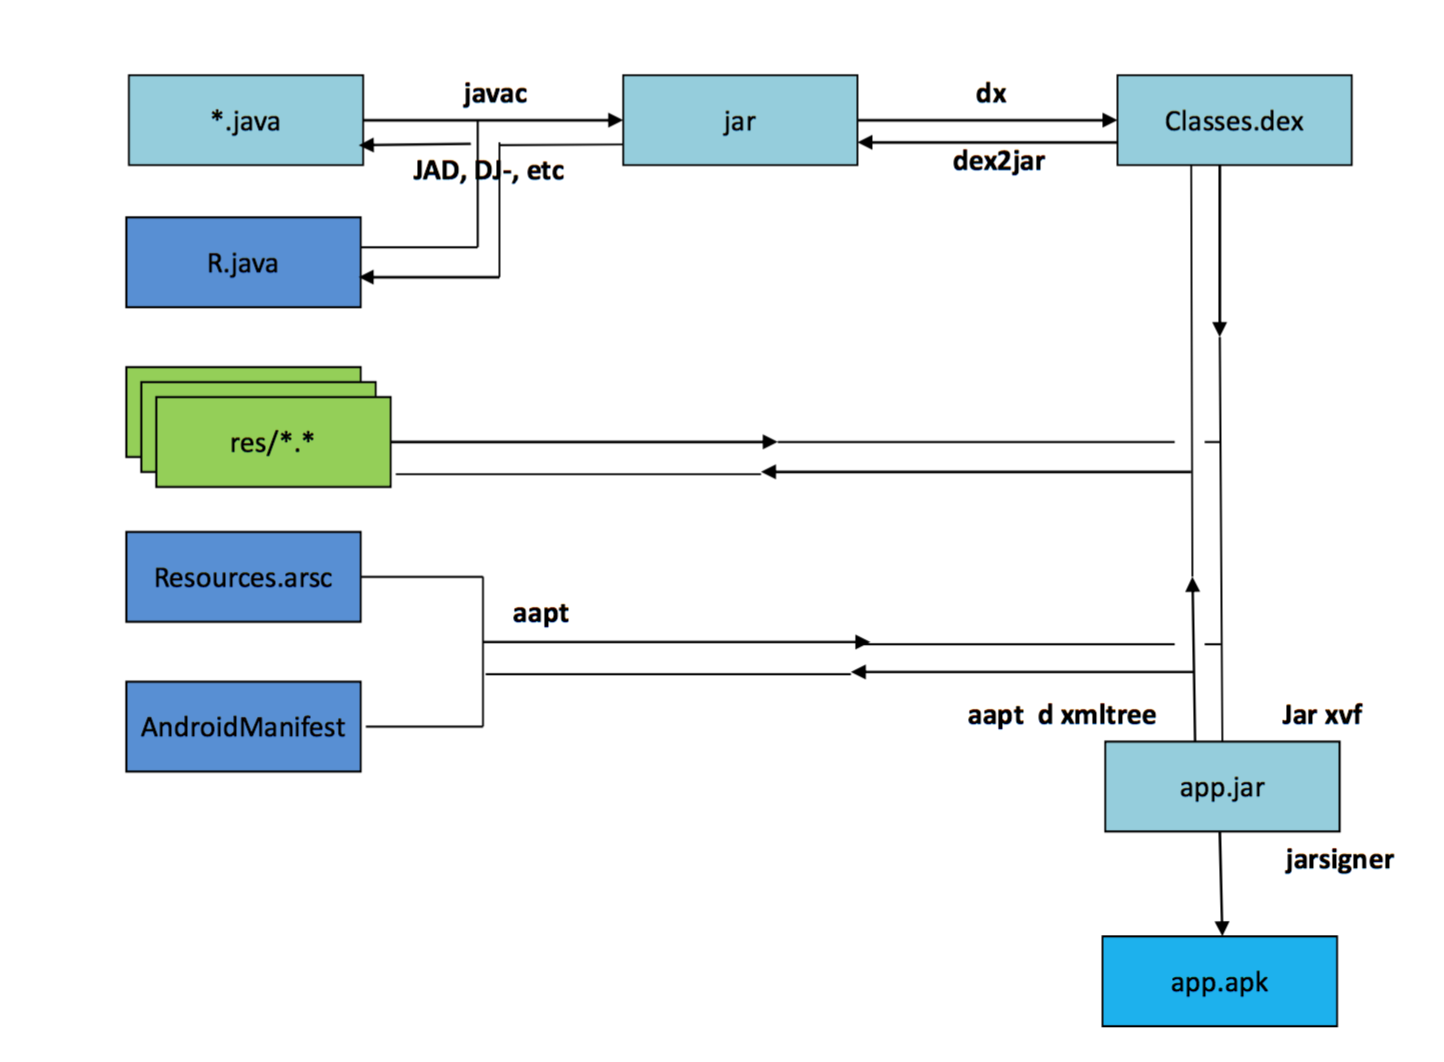
\includegraphics[width=0.8\textwidth]{data/re2.png}
    \caption{Overview of build and reverse engineering of an \gls{apk} \cite{andevconDalvikART}}
    \label{fig:re2}
\end{figure}
\cite{andevconDalvikART}
%

%
android vulnerability of app is reverse engineering the source code, patching security mechanism and recompiling the app
best case scenario is obtaining one to one copy of original source code since reading and understanding high level code is easiest so will the patching be
reality often not possible due various protecting of source code, also unnecessary since lower level representation of source code mgiht be enough to reveal mechanism
patch and compile low level code tools and documentation have matured

many tools and techniques

gaining information about a program and its implementation
details, process aims at enabling an analyst to understand the concrete
relation between implementation and functionality, optimal output
of such a process would be the original source code of the application, not possible in general\newline
Therefore, it is necessary for such a process to provide on the one hand abstract information about structure and inter-dependencies and on the other hand result in very detailed information like bytecode and mnemonics that allow interpretation of implementation\newline
hoffentlich starting points für investigations\newline
java, e.g. read the program code faster\newline


was ist reengineering? wie funktioniert es? was ist das ziel?\newline
reverse engineering process makes use of a whole range of different analysis
methodologies and tools.\newline
only consider static analysis tools\newline

IN ORDER TO GET FULL OVERVIEW DEX/SMALI/JAVA -see- WARUM?\newline

WAS MACHEN DIE TOOLS IM ALLGEMEINEN? WOZU BENUTZEN WIR SIE?\newline

• It comes as no surprise that .dex and .class are isomorphic
• DEX debug items map DEX offsets to Java line numbers
• Dex2jar tool can easily “decompile" from .dex back to a .jar
•  Extremely useful for reverse engineering – Evenmoresousefulformaliceandmischief

• Flow from DEX to JAVA is bidirectional, meaning that an attacker can:
• Decompile your code back to Java
• Remove annoyances like ads, registration
• Uncover sensitive data (app logic, or poorly guarded secrets)
• Replace certain classes with others, potentially malicious ones
• Recompile back to JAR, then DEX
• Put cloned/trojaned version of your app on Play or another market
• ASEC/OBB “solutions" for this fail miserably when target device is rooted.


\url{https://mobilesecuritywiki.com/}\newline
\url{https://net.cs.uni-bonn.de/fileadmin/user_upload/plohmann/2012-Schulz-Code_Protection_in_Android.pdf}\newline
main tools\newline
